\documentclass[aspectratio=169]{beamer}
% Add slides directory to search path for Dartmouth theme
\makeatletter
\def\input@path{{../}}
\makeatother
\usetheme{Dartmouth}
\usepackage{graphicx}
\usepackage{tikz}
\usepackage{amsmath}
\usepackage{listings}
\usepackage{xcolor}
\usepackage{booktabs}
% Code listing setup
\lstset{
  basicstyle=\ttfamily\small,
  keywordstyle=\color{blue},
  commentstyle=\color{gray},
  stringstyle=\color{red},
  showstringspaces=false,
  breaklines=true,
  frame=single,
  language=Python
}

\title{Dimensionality Reduction for NLP}
\subtitle{Lecture 10: PCA, t-SNE, and UMAP}
\author{PSYC 51.07: Models of Language and Communication - Week 4}
\date{Winter 2026}

\begin{document}

% ============================================================
% TITLE SLIDE
% ============================================================
\begin{frame}[shrink=10]
\titlepage
\end{frame}

% ============================================================
% OVERVIEW
% ============================================================
\begin{frame}[shrink=10]{Today's Lecture 📋}
\large
\begin{enumerate}\setlength{\itemsep}{0pt}
    \item 📉 \textbf{The Curse of Dimensionality}
    \item 📊 \textbf{Principal Component Analysis (PCA)}
    \item 🎨 \textbf{t-SNE: Stochastic Neighbor Embedding}
    \item 🗺️ \textbf{UMAP: Uniform Manifold Approximation}
    \item 🔍 \textbf{Comparison \& Best Practices}
    \item 💻 \textbf{Visualization Techniques}
\end{enumerate}

\vspace{1em}
\textit{Goal: Learn to visualize and explore high-dimensional embeddings}
\end{frame}

% ============================================================
% CURSE OF DIMENSIONALITY
% ============================================================
\begin{frame}[shrink=10]{The Curse of Dimensionality 📉}
\textbf{The Problem:}

\vspace{1em}

\begin{columns}[T]
\begin{column}{0.48\textwidth}
\textbf{Word Embeddings:}
\begin{itemize}\setlength{\itemsep}{0pt}
    \item Word2Vec: 300 dimensions
    \item GloVe: 300 dimensions
    \item FastText: 300 dimensions
    \item BERT: 768 dimensions
    \item GPT-3: 12,288 dimensions!
\end{itemize}

\vspace{0.5em}
\textbf{Challenges:}
\begin{itemize}\setlength{\itemsep}{0pt}
    \item Can't visualize 300D space
    \item Distances behave strangely
    \item Computation expensive
    \item Storage requirements
    \item Interpretation difficult
\end{itemize}
\end{column}

\begin{column}{0.48\textwidth}
\textbf{Interesting Properties:}
\begin{itemize}\setlength{\itemsep}{0pt}
    \item In high dimensions, most points are far apart
    \item Volume concentrates in corners
    \item Random vectors nearly orthogonal
    \item Nearest neighbors may not be near!
\end{itemize}

\vspace{1em}
\begin{exampleblock}{Example}
In 300D space with uniform distribution:
\begin{itemize}\setlength{\itemsep}{0pt}
    \item Expected distance to nearest neighbor: $\approx$ distance to farthest!
    \item All points approximately equidistant
\end{itemize}
\end{exampleblock}
\end{column}
\end{columns}

\vspace{1em}
\begin{center}
\Large
\alert{Solution: Dimensionality Reduction}
\end{center}
\end{frame}

% ============================================================
% WHY REDUCE
% ============================================================
\begin{frame}[shrink=10]{Why Dimensionality Reduction? 🎯}
\small
\begin{columns}[T]
\begin{column}{0.48\textwidth}
\textbf{Visualization:}
\begin{itemize}\setlength{\itemsep}{0pt}
    \item 2D/3D plots
    \item Explore semantic structure
    \item Identify clusters
    \item Discover patterns
    \item Quality assurance
\end{itemize}

\vspace{0.5em}
\textbf{Computation:}
\begin{itemize}\setlength{\itemsep}{0pt}
    \item Faster algorithms
    \item Less memory
    \item Enable real-time systems
    \item Scalability
\end{itemize}
\end{column}

\begin{column}{0.48\textwidth}
\textbf{Machine Learning:}
\begin{itemize}\setlength{\itemsep}{0pt}
    \item Reduce overfitting
    \item Feature selection
    \item Improve generalization
    \item Remove noise
    \item Combat curse of dimensionality
\end{itemize}

\vspace{0.5em}
\textbf{Interpretation:}
\begin{itemize}\setlength{\itemsep}{0pt}
    \item Understand relationships
    \item Identify important dimensions
    \item Communicate results
    \item Debug models
\end{itemize}
\end{column}
\end{columns}

\vspace{1em}

\begin{block}{The Goal}
Reduce from $d$ dimensions (e.g., 300) to $k$ dimensions (e.g., 2 or 3) while \alert{preserving important structure}
\end{block}
\end{frame}

% ============================================================
% PCA INTRO
% ============================================================
\begin{frame}[shrink=10]{Principal Component Analysis (PCA) 📊}
\textbf{The classic linear dimensionality reduction method}

\vspace{1em}

\begin{columns}[T]
\begin{column}{0.48\textwidth}
\textbf{Intuition:}
\begin{itemize}\setlength{\itemsep}{0pt}
    \item Find directions of maximum variance
    \item Project data onto these directions
    \item First PC: most variance
    \item Second PC: second most (orthogonal)
    \item And so on...
\end{itemize}

\vspace{0.5em}
\textbf{Properties:}
\begin{itemize}\setlength{\itemsep}{0pt}
    \item Linear transformation
    \item Preserves global structure
    \item Deterministic
    \item Fast computation
    \item Interpretable (sometimes)
\end{itemize}
\end{column}

\begin{column}{0.48\textwidth}
\begin{center}
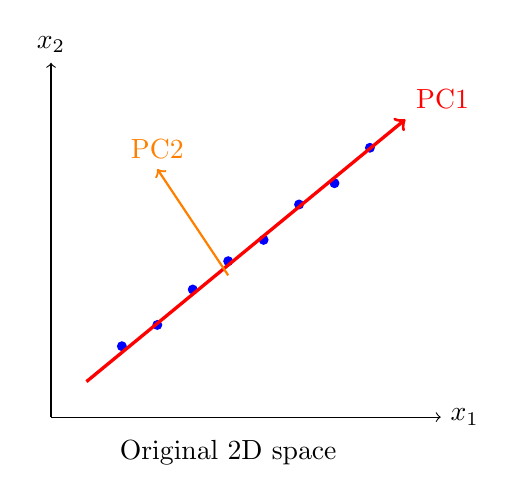
\begin{tikzpicture}[scale=0.9]
    % Data points
    \foreach \x/\y in {1/1, 1.5/1.3, 2/1.8, 2.5/2.2, 3/2.5, 3.5/3, 4/3.3, 4.5/3.8}
        \fill[blue] (\x,\y) circle (2pt);

    % Principal components
    \draw[->, very thick, red] (0.5,0.5) -- (5,4.2) node[above right] {PC1};
    \draw[->, thick, orange] (2.5,2) -- (1.5,3.5) node[above] {PC2};

    % Axes
    \draw[->] (0,0) -- (5.5,0) node[right] {$x_1$};
    \draw[->] (0,0) -- (0,5) node[above] {$x_2$};

    % Labels
    \node at (2.5, -0.5) {Original 2D space};
\end{tikzpicture}
\end{center}

\vspace{0.5em}
PC1 captures most variation

PC2 captures remaining variation (orthogonal to PC1)
\end{column}
\end{columns}
\end{frame}

% ============================================================
% PCA ALGORITHM
% ============================================================
\begin{frame}[shrink=10]{PCA: The Algorithm 🔧}
\textbf{Mathematical formulation:}

\vspace{1em}

\begin{enumerate}\setlength{\itemsep}{0pt}
    \item \textbf{Center the data:}
    \begin{itemize}\setlength{\itemsep}{0pt}
        \item Subtract mean: $\tilde{X} = X - \bar{X}$
        \item Each dimension has mean 0
    \end{itemize}

    \item \textbf{Compute covariance matrix:}
    \begin{itemize}\setlength{\itemsep}{0pt}
        \item $C = \frac{1}{n-1} \tilde{X}^T \tilde{X}$
        \item Captures correlations between dimensions
    \end{itemize}

    \item \textbf{Eigenvalue decomposition:}
    \begin{itemize}\setlength{\itemsep}{0pt}
        \item $C = V \Lambda V^T$
        \item $V$: eigenvectors (principal components)
        \item $\Lambda$: eigenvalues (variance explained)
    \end{itemize}

    \item \textbf{Project onto top k eigenvectors:}
    \begin{itemize}\setlength{\itemsep}{0pt}
        \item Sort by eigenvalues (descending)
        \item Keep top $k$: $V_k$
        \item Project: $X_{reduced} = \tilde{X} V_k$
    \end{itemize}
\end{enumerate}

\vspace{1em}

\textbf{Variance explained:} $\frac{\sum_{i=1}^k \lambda_i}{\sum_{i=1}^d \lambda_i}$
\end{frame}

% ============================================================
% PCA CODE
% ============================================================
\begin{frame}[fragile]{PCA in Practice 💻}
\begin{lstlisting}[language=Python]
from sklearn.decomposition import PCA
from sklearn.preprocessing import StandardScaler
import numpy as np
import matplotlib.pyplot as plt

# Assume we have word embeddings: shape (vocab_size, 300)
# For example, Word2Vec embeddings

# Standardize the data (optional but recommended)
scaler = StandardScaler()
embeddings_scaled = scaler.fit_transform(embeddings)

# Apply PCA
pca = PCA(n_components=2)  # Reduce to 2D for visualization
embeddings_2d = pca.fit_transform(embeddings_scaled)

# Check variance explained
print(f"Variance explained: {pca.explained_variance_ratio_}")
print(f"Total: {sum(pca.explained_variance_ratio_):.2%}")

# Visualize
plt.figure(figsize=(10, 8))
plt.scatter(embeddings_2d[:, 0], embeddings_2d[:, 1], alpha=0.5)

# Annotate some words
words = ['king', 'queen', 'man', 'woman', 'cat', 'dog']
for word in words:
    idx = word_to_idx[word]
    plt.annotate(word, (embeddings_2d[idx, 0], embeddings_2d[idx, 1]))

plt.xlabel('PC1')
plt.ylabel('PC2')
plt.title('Word Embeddings - PCA Projection')
plt.show()
\end{lstlisting}
\end{frame}

% ============================================================
% PCA LIMITATIONS
% ============================================================
\begin{frame}[shrink=10]{PCA Limitations ⚠️}
\begin{columns}[T]
\begin{column}{0.48\textwidth}
\textbf{Assumes Linearity:}
\begin{itemize}\setlength{\itemsep}{0pt}
    \item Only captures linear relationships
    \item Word embeddings often have non-linear structure
    \item May miss important patterns
\end{itemize}

\vspace{0.5em}
\begin{center}
\begin{tikzpicture}[scale=0.7]
    % Swiss roll data (can't be linearized)
    \foreach \t in {0,0.2,...,6.28} {
        \pgfmathsetmacro{\x}{\t * cos(\t r)}
        \pgfmathsetmacro{\y}{\t * sin(\t r)}
        \fill[blue] (\x, \y) circle (1.5pt);
    }
    \node at (0, -3) {Non-linear manifold};
    \node at (0, -3.5) {\small PCA struggles here!};
\end{tikzpicture}
\end{center}
\end{column}

\begin{column}{0.48\textwidth}
\textbf{Other Issues:}
\begin{itemize}\setlength{\itemsep}{0pt}
    \item \textbf{Variance ≠ Importance:}
    \begin{itemize}\setlength{\itemsep}{0pt}
        \item Preserves variance, not semantic structure
        \item Noisy dimensions may have high variance
    \end{itemize}

    \item \textbf{Global focus:}
    \begin{itemize}\setlength{\itemsep}{0pt}
        \item May lose local structure
        \item Clusters can become blurred
    \end{itemize}

    \item \textbf{Interpretability:}
    \begin{itemize}\setlength{\itemsep}{0pt}
        \item PCs are linear combinations
        \item Hard to interpret semantically
    \end{itemize}
\end{itemize}

\vspace{1em}
\begin{alertblock}{When to Use PCA}
\begin{itemize}\setlength{\itemsep}{0pt}
    \item Quick first exploration
    \item Preprocessing for other methods
    \item When speed is critical
    \item Linear structure expected
\end{itemize}
\end{alertblock}
\end{column}
\end{columns}
\end{frame}

% ============================================================
% TSNE INTRO
% ============================================================
\begin{frame}[shrink=10]{t-SNE: t-Distributed Stochastic Neighbor Embedding 🎨}
\textbf{Non-linear dimensionality reduction for visualization}

\vspace{1em}

\begin{columns}[T]
\begin{column}{0.48\textwidth}
\textbf{Key Idea:}
\begin{itemize}\setlength{\itemsep}{0pt}
    \item Model similarity as probability
    \item High-D: Gaussian similarity
    \item Low-D: t-distribution similarity
    \item Minimize divergence between them
    \item Preserves \alert{local structure}
\end{itemize}

\vspace{0.5em}
\textbf{Advantages:}
\begin{itemize}\setlength{\itemsep}{0pt}
    \item Beautiful visualizations
    \item Reveals clusters
    \item Non-linear mappings
    \item Great for exploration
    \item Widely used in practice
\end{itemize}
\end{column}

\begin{column}{0.48\textwidth}
\textbf{How it works:}

\vspace{0.3em}
\begin{enumerate}\setlength{\itemsep}{0pt}
    \item Compute pairwise similarities in high-D:
    \begin{align*}
    p_{j|i} = \frac{\exp(-||x_i - x_j||^2 / 2\sigma_i^2)}{\sum_{k \neq i} \exp(-||x_i - x_k||^2 / 2\sigma_i^2)}
    \end{align*}

    \item Compute similarities in low-D using t-distribution:
    \begin{align*}
    q_{ij} = \frac{(1 + ||y_i - y_j||^2)^{-1}}{\sum_{k \neq l}(1 + ||y_k - y_l||^2)^{-1}}
    \end{align*}

    \item Minimize KL divergence:
    \begin{align*}
    C = \sum_i KL(P_i || Q_i)
    \end{align*}

    \item Use gradient descent to optimize $y_i$
\end{enumerate}
\end{column}
\end{columns}

\vspace{0.5em}
\small
\textit{Reference: van der Maaten \& Hinton (2008). "Visualizing Data using t-SNE"}
\end{frame}

% ============================================================
% TSNE DETAILS
% ============================================================
\begin{frame}[shrink=10]{t-SNE: Key Concepts 🔍}
\textbf{Why t-distribution in low-D?}

\vspace{1em}

\begin{columns}[T]
\begin{column}{0.48\textwidth}
\textbf{Crowding Problem:}
\begin{itemize}\setlength{\itemsep}{0pt}
    \item High-D: many points at medium distance
    \item Low-D: not enough space
    \item Gaussian would squash together
    \item t-distribution has heavier tails
    \item Allows distant points to stay apart
\end{itemize}

\vspace{1em}
\begin{center}
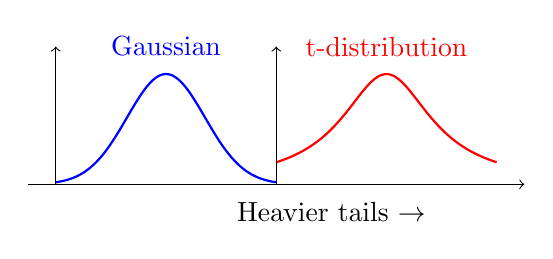
\begin{tikzpicture}[scale=0.7]
    % Gaussian
    \draw[blue, thick, domain=-2:2, samples=100] plot (\x, {2*exp(-\x*\x)});
    \node[blue] at (0, 2.5) {Gaussian};

    % t-distribution
    \draw[red, thick, domain=-2:2, samples=100] plot (\x+4, {2/(1+\x*\x)});
    \node[red] at (4, 2.5) {t-distribution};

    % Axes
    \draw[->] (-2.5,0) -- (6.5,0);
    \draw[->] (-2,0) -- (-2,2.5);
    \draw[->] (2,0) -- (2,2.5);

    \node at (3, -0.5) {Heavier tails $\rightarrow$};
\end{tikzpicture}
\end{center}
\end{column}

\begin{column}{0.48\textwidth}
\textbf{Hyperparameters:}

\vspace{0.3em}
\textbf{1. Perplexity (most important):}
\begin{itemize}\setlength{\itemsep}{0pt}
    \item Roughly: number of nearest neighbors
    \item Typical: 5-50
    \item Small dataset: 5-20
    \item Large dataset: 30-50
    \item \alert{Different values = different results!}
\end{itemize}

\vspace{0.5em}
\textbf{2. Number of iterations:}
\begin{itemize}\setlength{\itemsep}{0pt}
    \item Minimum: 1000
    \item Recommended: 2000-5000
    \item More = better (but slower)
\end{itemize}

\vspace{0.5em}
\textbf{3. Learning rate:}
\begin{itemize}\setlength{\itemsep}{0pt}
    \item Typical: 10-1000
    \item Default: 200
    \item May need tuning
\end{itemize}
\end{column}
\end{columns}
\end{frame}

% ============================================================
% TSNE CODE
% ============================================================
\begin{frame}[fragile]{t-SNE in Practice 💻}
\begin{lstlisting}[language=Python]
from sklearn.manifold import TSNE
import matplotlib.pyplot as plt

# Apply t-SNE (can be slow for large datasets)
tsne = TSNE(
    n_components=2,      # 2D visualization
    perplexity=30,       # try 5-50
    n_iter=2000,         # iterations
    random_state=42,     # reproducibility
    verbose=1            # show progress
)

embeddings_2d = tsne.fit_transform(embeddings)

# Visualize with labels
plt.figure(figsize=(12, 10))

# Color by semantic category (if available)
categories = ['animals', 'food', 'technology', ...]
colors = ['red', 'blue', 'green', ...]

for cat, color in zip(categories, colors):
    mask = labels == cat
    plt.scatter(
        embeddings_2d[mask, 0],
        embeddings_2d[mask, 1],
        c=color,
        label=cat,
        alpha=0.6
    )

# Annotate some words
for word, idx in word_to_idx.items():
    if word in important_words:
        plt.annotate(
            word,
            (embeddings_2d[idx, 0], embeddings_2d[idx, 1])
        )

plt.legend()
plt.title('Word Embeddings - t-SNE Projection')
plt.show()
\end{lstlisting}
\end{frame}

% ============================================================
% TSNE LIMITATIONS
% ============================================================
\begin{frame}[shrink=10]{t-SNE Limitations and Caveats ⚠️}
\begin{enumerate}\setlength{\itemsep}{0pt}
    \item \textbf{Slow:}
    \begin{itemize}\setlength{\itemsep}{0pt}
        \item $O(n^2)$ complexity
        \item Prohibitive for $>$10k points
        \item Solution: Use PCA first to reduce to 50D, then t-SNE
    \end{itemize}

    \item \textbf{Non-deterministic:}
    \begin{itemize}\setlength{\itemsep}{0pt}
        \item Different runs $\rightarrow$ different results
        \item Random initialization matters
        \item Set random seed for reproducibility
    \end{itemize}

    \item \textbf{Hyperparameter sensitive:}
    \begin{itemize}\setlength{\itemsep}{0pt}
        \item Perplexity dramatically affects results
        \item No "correct" value
        \item Need to try multiple values
    \end{itemize}

    \item \textbf{Interpretation pitfalls:}
    \begin{itemize}\setlength{\itemsep}{0pt}
        \item \alert{Distances between clusters are meaningless!}
        \item Only local structure is preserved
        \item Cluster sizes can be misleading
        \item Don't over-interpret global structure
    \end{itemize}

    \item \textbf{Not for dimensionality reduction in ML:}
    \begin{itemize}\setlength{\itemsep}{0pt}
        \item No out-of-sample extension
        \item Can't transform new points
        \item Use only for visualization!
    \end{itemize}
\end{enumerate}
\end{frame}

% ============================================================
% UMAP INTRO
% ============================================================
\begin{frame}[shrink=10]{UMAP: Uniform Manifold Approximation \& Projection 🗺️}
\textbf{Modern alternative to t-SNE (2018)}

\vspace{1em}

\begin{columns}[T]
\begin{column}{0.48\textwidth}
\textbf{Key Advantages over t-SNE:}
\begin{itemize}\setlength{\itemsep}{0pt}
    \item \alert{Much faster} ($O(n \log n)$ vs $O(n^2)$)
    \item Preserves \alert{both} local and global structure
    \item Can transform new points
    \item Theoretically grounded (topology)
    \item Scales to millions of points
    \item More robust hyperparameters
\end{itemize}

\vspace{0.5em}
\textbf{When to Use:}
\begin{itemize}\setlength{\itemsep}{0pt}
    \item Large datasets ($>$10k points)
    \item Need global structure
    \item Production systems
    \item Consistent results important
    \item Most NLP visualization tasks!
\end{itemize}
\end{column}

\begin{column}{0.48\textwidth}
\textbf{How it Works:}

\vspace{0.3em}
\begin{enumerate}\setlength{\itemsep}{0pt}
    \item Construct fuzzy topological representation of high-D data
    \item Find low-D representation with similar topology
    \item Use Riemannian geometry
    \item Optimize cross-entropy loss
\end{enumerate}

\vspace{0.5em}
\textbf{Main Hyperparameters:}

\vspace{0.3em}
\textbf{1. n\_neighbors (15):}
\begin{itemize}\setlength{\itemsep}{0pt}
    \item Local vs. global balance
    \item Small: local structure
    \item Large: global structure
\end{itemize}

\vspace{0.3em}
\textbf{2. min\_dist (0.1):}
\begin{itemize}\setlength{\itemsep}{0pt}
    \item How tightly to pack points
    \item Small: tight clusters
    \item Large: loose, spread out
\end{itemize}
\end{column}
\end{columns}

\vspace{0.5em}
\small
\textit{Reference: McInnes \& Healy (2018). "UMAP: Uniform Manifold Approximation and Projection"}
\end{frame}

% ============================================================
% UMAP CODE
% ============================================================
\begin{frame}[fragile]{UMAP in Practice 💻}
\begin{lstlisting}[language=Python]
import umap
import matplotlib.pyplot as plt

# Apply UMAP
reducer = umap.UMAP(
    n_components=2,      # 2D visualization
    n_neighbors=15,      # local/global balance (try 5-50)
    min_dist=0.1,        # cluster tightness (try 0.0-0.99)
    metric='cosine',     # good for word embeddings
    random_state=42
)

embeddings_2d = reducer.fit_transform(embeddings)

# Can also transform new points! (unlike t-SNE)
new_embeddings_2d = reducer.transform(new_embeddings)

# Visualize
plt.figure(figsize=(12, 10))
scatter = plt.scatter(
    embeddings_2d[:, 0],
    embeddings_2d[:, 1],
    c=cluster_labels,     # color by cluster
    cmap='Spectral',
    s=5,
    alpha=0.6
)
plt.colorbar(scatter)

# Annotate
for word in important_words:
    idx = word_to_idx[word]
    plt.annotate(
        word,
        (embeddings_2d[idx, 0], embeddings_2d[idx, 1]),
        fontsize=12
    )

plt.title('Word Embeddings - UMAP Projection')
plt.show()
\end{lstlisting}
\end{frame}

% ============================================================
% COMPARISON
% ============================================================
\begin{frame}{PCA vs. t-SNE vs. UMAP 🔍}
\begin{center}
\begin{tabular}{lccc}
\toprule
\textbf{Property} & \textbf{PCA} & \textbf{t-SNE} & \textbf{UMAP} \\
\midrule
Linear/Non-linear & Linear & Non-linear & Non-linear \\
Speed & Very Fast ⚡ & Slow 🐌 & Fast ⚡ \\
Scalability & Excellent & Poor ($<$10k) & Excellent \\
Global structure & ✓ & ✗ & ✓ \\
Local structure & $\sim$ & ✓ & ✓ \\
Deterministic & ✓ & ✗ & $\sim$ \\
Out-of-sample & ✓ & ✗ & ✓ \\
Hyperparameters & Few & Sensitive & Robust \\
Interpretation & Medium & Hard & Medium \\
\textbf{Best for NLP} & Preprocessing & Small viz & \textbf{Most tasks} \\
\bottomrule
\end{tabular}
\end{center}

\vspace{1em}

\begin{block}{Recommendations}
\begin{itemize}\setlength{\itemsep}{0pt}
    \item \textbf{PCA}: Quick first pass, preprocessing, need speed
    \item \textbf{t-SNE}: Small datasets ($<$10k), only care about local clusters
    \item \textbf{UMAP}: \alert{Default choice!} Fast, scalable, preserves structure
\end{itemize}
\end{block}

\vspace{0.5em}
\textbf{Common workflow:} PCA to 50D $\rightarrow$ UMAP to 2D for visualization
\end{frame}

% ============================================================
% VISUALIZATION BEST PRACTICES
% ============================================================
\begin{frame}[shrink=10]{Visualization Best Practices 🎨}
\begin{enumerate}\setlength{\itemsep}{0pt}
    \item \textbf{Preprocessing:}
    \begin{itemize}\setlength{\itemsep}{0pt}
        \item Standardize features (mean=0, std=1)
        \item Remove outliers (optional)
        \item For very large datasets: sample or use PCA first
    \end{itemize}

    \item \textbf{Try multiple hyperparameters:}
    \begin{itemize}\setlength{\itemsep}{0pt}
        \item t-SNE perplexity: 5, 10, 30, 50
        \item UMAP n\_neighbors: 5, 15, 30, 50
        \item Different views reveal different structure
    \end{itemize}

    \item \textbf{Color intelligently:}
    \begin{itemize}\setlength{\itemsep}{0pt}
        \item By semantic category
        \item By cluster assignment
        \item By frequency (size)
        \item By POS tag, domain, etc.
    \end{itemize}

    \item \textbf{Interactive visualization:}
    \begin{itemize}\setlength{\itemsep}{0pt}
        \item Use plotly, bokeh for interactivity
        \item Hover tooltips with word info
        \item Zoom and pan
        \item Filter by category
    \end{itemize}

    \item \textbf{Annotate selectively:}
    \begin{itemize}\setlength{\itemsep}{0pt}
        \item Too many labels = clutter
        \item Show representative words
        \item Use repel/adjust\_text to avoid overlap
    \end{itemize}
\end{enumerate}
\end{frame}

% ============================================================
% INTERACTIVE VIZ CODE
% ============================================================
\begin{frame}[fragile]{Interactive Visualization 💡}
\begin{lstlisting}[language=Python]
import plotly.express as px
import plotly.graph_objects as go
import pandas as pd

# Prepare data
df = pd.DataFrame({
    'x': embeddings_2d[:, 0],
    'y': embeddings_2d[:, 1],
    'word': words,
    'category': categories,
    'frequency': frequencies
})

# Create interactive plot with plotly
fig = px.scatter(
    df,
    x='x',
    y='y',
    color='category',
    size='frequency',
    hover_data=['word', 'frequency'],
    title='Word Embeddings (UMAP)',
    width=1000,
    height=800
)

# Add text annotations for important words
for word in important_words:
    row = df[df['word'] == word].iloc[0]
    fig.add_annotation(
        x=row['x'],
        y=row['y'],
        text=word,
        showarrow=False,
        font=dict(size=12)
    )

# Show
fig.show()

# Can also save as HTML
fig.write_html('embeddings_viz.html')
\end{lstlisting}
\end{frame}

% ============================================================
% APPLICATIONS
% ============================================================
\begin{frame}[shrink=10]{Applications in NLP 🚀}
\begin{enumerate}\setlength{\itemsep}{0pt}
    \item \textbf{Embedding Quality Assessment:}
    \begin{itemize}\setlength{\itemsep}{0pt}
        \item Visualize to check if similar words cluster
        \item Identify anomalies and outliers
        \item Compare different embedding methods
        \item Debugging and quality control
    \end{itemize}

    \item \textbf{Exploratory Data Analysis:}
    \begin{itemize}\setlength{\itemsep}{0pt}
        \item Discover themes in corpus
        \item Identify semantic groupings
        \item Find polysemous words (appear in multiple clusters)
        \item Understand domain vocabulary
    \end{itemize}

    \item \textbf{Topic Modeling Visualization:}
    \begin{itemize}\setlength{\itemsep}{0pt}
        \item Visualize document embeddings
        \item Show topic distributions
        \item Interactive topic browsers (pyLDAvis, BERTopic viz)
    \end{itemize}

    \item \textbf{Model Interpretation:}
    \begin{itemize}\setlength{\itemsep}{0pt}
        \item Visualize attention patterns
        \item Show layer representations in transformers
        \item Understand what models learn
    \end{itemize}

    \item \textbf{Presentation \& Communication:}
    \begin{itemize}\setlength{\itemsep}{0pt}
        \item Explain models to stakeholders
        \item Publication figures
        \item Teaching and demos
    \end{itemize}
\end{enumerate}
\end{frame}

% ============================================================
% CASE STUDY
% ============================================================
\begin{frame}[fragile]{Case Study: Visualizing BERT Layers 🔬}
\textbf{Question:} What do different BERT layers capture?

\vspace{1em}

\begin{columns}[T]
\begin{column}{0.48\textwidth}
\textbf{Approach:}
\begin{enumerate}\setlength{\itemsep}{0pt}
    \item Extract embeddings from each layer
    \item Apply UMAP to each layer separately
    \item Visualize and compare
\end{enumerate}

\vspace{0.5em}
\textbf{Typical Findings:}
\begin{itemize}\setlength{\itemsep}{0pt}
    \item \textbf{Layer 0-2:} Syntactic (POS tags cluster)
    \item \textbf{Layer 3-8:} Semantic (meaning clusters)
    \item \textbf{Layer 9-12:} Task-specific
\end{itemize}

\vspace{0.5em}
\textbf{Insights:}
\begin{itemize}\setlength{\itemsep}{0pt}
    \item Lower layers: syntax
    \item Middle layers: semantics
    \item Upper layers: task adaptation
    \item Confirms linguistic hierarchy
\end{itemize}
\end{column}

\begin{column}{0.48\textwidth}
\begin{lstlisting}[language=Python]
from transformers import BertModel, BertTokenizer

model = BertModel.from_pretrained('bert-base-uncased', output_hidden_states=True)
tokenizer = BertTokenizer.from_pretrained('bert-base-uncased')

# Get embeddings from all layers
tokens = tokenizer(sentences, return_tensors='pt', padding=True)
outputs = model(**tokens)

# outputs.hidden_states: tuple of 13 tensors
# (embedding layer + 12 transformer layers)

for layer_idx in range(13):
    layer_embeddings = outputs.hidden_states[layer_idx]

    # Average over sequence length
    avg_embeddings = layer_embeddings.mean(dim=1).numpy()

    # Apply UMAP
    reducer = umap.UMAP(n_components=2)
    viz_2d = reducer.fit_transform(avg_embeddings)

    # Plot
    plt.figure()
    plt.scatter(viz_2d[:, 0], viz_2d[:, 1], c=pos_tags)
    plt.title(f'Layer {layer_idx}')
    plt.show()
\end{lstlisting}
\end{column}
\end{columns}

\vspace{0.5em}
\small
\textit{Reference: Jawahar et al. (2019). "What Does BERT Learn about the Structure of Language?"}
\end{frame}

% ============================================================
% DISCUSSION
% ============================================================
\begin{frame}[shrink=10]{Discussion Question 💬}
\begin{center}
\Large
\textbf{What does a 2D visualization actually tell us about 300D space?}
\end{center}

\vspace{1em}

\textbf{Consider:}
\begin{itemize}\setlength{\itemsep}{0pt}
    \item We compress 300 dimensions into 2
    \item Massive information loss (>99\%)
    \item Different methods show different views
    \item Hyperparameters change the story
\end{itemize}

\vspace{1em}

\begin{columns}[T]
\begin{column}{0.48\textwidth}
\textbf{What we CAN conclude:}
\begin{itemize}\setlength{\itemsep}{0pt}
    \item Rough semantic groupings
    \item Relative proximities
    \item Cluster existence
    \item Outliers and anomalies
    \item Qualitative patterns
\end{itemize}
\end{column}

\begin{column}{0.48\textwidth}
\textbf{What we CANNOT conclude:}
\begin{itemize}\setlength{\itemsep}{0pt}
    \item Exact distances
    \item True high-D structure
    \item Cluster sizes (t-SNE)
    \item Between-cluster distances
    \item Quantitative relationships
\end{itemize}
\end{column}
\end{columns}

\vspace{1em}

\begin{alertblock}{Important}
Dimensionality reduction is a \alert{lossy transformation}. Always combine visualization with quantitative evaluation!
\end{alertblock}
\end{frame}

% ============================================================
% PRACTICAL TIPS
% ============================================================
\begin{frame}[shrink=10]{Practical Tips 💡}
\begin{enumerate}\setlength{\itemsep}{0pt}
    \item \textbf{Choose the right tool:}
    \begin{itemize}\setlength{\itemsep}{0pt}
        \item Default: UMAP (fast, balanced)
        \item Need speed: PCA
        \item Small dataset, only local: t-SNE
    \end{itemize}

    \item \textbf{Preprocessing matters:}
    \begin{itemize}\setlength{\itemsep}{0pt}
        \item StandardScaler for PCA
        \item Consider normalization for UMAP/t-SNE
        \item Remove extreme outliers
    \end{itemize}

    \item \textbf{Try multiple settings:}
    \begin{itemize}\setlength{\itemsep}{0pt}
        \item Run with different hyperparameters
        \item Compare results
        \item Don't cherry-pick!
    \end{itemize}

    \item \textbf{Use color wisely:}
    \begin{itemize}\setlength{\itemsep}{0pt}
        \item Semantic categories
        \item Continuous values (frequency, sentiment)
        \item Consider colorblind-friendly palettes
    \end{itemize}

    \item \textbf{Save your random seeds:}
    \begin{itemize}\setlength{\itemsep}{0pt}
        \item Makes results reproducible
        \item Important for publications
        \item Helps debugging
    \end{itemize}

    \item \textbf{Computational tips:}
    \begin{itemize}\setlength{\itemsep}{0pt}
        \item For $>$100k points: PCA first to 50D, then UMAP
        \item Use n\_jobs=-1 for parallel computation
        \item Consider approximate nearest neighbors (Annoy, FAISS)
    \end{itemize}
\end{enumerate}
\end{frame}

% ============================================================
% SUMMARY
% ============================================================
\begin{frame}[shrink=10]{Summary 🎯}
\textbf{What we learned today:}

\begin{enumerate}\setlength{\itemsep}{0pt}
    \item \textbf{Curse of Dimensionality:} High-D space is weird, need reduction

    \item \textbf{PCA:}
    \begin{itemize}\setlength{\itemsep}{0pt}
        \item Linear, fast, preserves global structure
        \item Good for preprocessing and quick exploration
    \end{itemize}

    \item \textbf{t-SNE:}
    \begin{itemize}\setlength{\itemsep}{0pt}
        \item Non-linear, preserves local structure
        \item Beautiful visualizations but slow
        \item Sensitive to hyperparameters
    \end{itemize}

    \item \textbf{UMAP:}
    \begin{itemize}\setlength{\itemsep}{0pt}
        \item Fast, scalable, balanced local+global
        \item Best default choice for NLP
        \item Can transform new points
    \end{itemize}

    \item \textbf{Best Practices:}
    \begin{itemize}\setlength{\itemsep}{0pt}
        \item Try multiple methods and parameters
        \item Use interactive visualizations
        \item Don't over-interpret 2D projections
    \end{itemize}
\end{enumerate}

\vspace{0.5em}
\begin{center}
\textbf{Next: Cognitive models of semantic representation!}
\end{center}
\end{frame}

% ============================================================
% REFERENCES
% ============================================================
\begin{frame}[shrink=10]{Key References 📚}
\small
\textbf{Foundational Papers:}
\begin{itemize}\setlength{\itemsep}{0pt}
    \item Pearson, K. (1901). "On Lines and Planes of Closest Fit to Systems of Points in Space" (PCA)
    \item van der Maaten \& Hinton (2008). "Visualizing Data using t-SNE"
    \item McInnes et al. (2018). "UMAP: Uniform Manifold Approximation and Projection for Dimension Reduction"
\end{itemize}

\vspace{0.5em}
\textbf{Applications:}
\begin{itemize}\setlength{\itemsep}{0pt}
    \item Jawahar et al. (2019). "What Does BERT Learn about the Structure of Language?"
    \item Coenen et al. (2019). "Visualizing and Measuring the Geometry of BERT"
\end{itemize}

\vspace{0.5em}
\textbf{Guides \& Tutorials:}
\begin{itemize}\setlength{\itemsep}{0pt}
    \item Wattenberg et al. (2016). "How to Use t-SNE Effectively" (Distill)
    \item UMAP documentation: \url{https://umap-learn.readthedocs.io/}
    \item Scikit-learn User Guide: \url{https://scikit-learn.org/stable/modules/manifold.html}
\end{itemize}

\vspace{0.5em}
\textbf{Tools:}
\begin{itemize}\setlength{\itemsep}{0pt}
    \item Scikit-learn: PCA, t-SNE
    \item UMAP-learn: \texttt{pip install umap-learn}
    \item Plotly: \texttt{pip install plotly}
\end{itemize}
\end{frame}

% ============================================================
% QUESTIONS
% ============================================================
\begin{frame}{Questions? 🙋}
\begin{center}
\LARGE
\textbf{Next Lecture:}

\vspace{1em}
Cognitive Models of Semantic Representation

\vspace{1em}
\textit{How do humans represent meaning?}
\end{center}
\end{frame}

\end{document}
